\newcommand{\einh}[1]{\mathrm{#1}}

%\title{Tutorial on Design Amplifiers based on S-Parameter Simulation}
%\maketitle
\tutsection{Introduction}

This tutorial shows how to design Amplifiers using QUCS \cite{qucs}
and the S-Parameter simulation as well as circle tools for gain and
noise. We will start with available transistors and design two
amplifiers: one single stage sub-GHz amplifier, which can be used for
cellular or short range radio applications. The second will be a dual
stage above ten GHz amplifier as it could be used in direct
broadcasting satellite applications. Different technologies and
topologies are used.

It is assumed that the reader is familiar with foundations of
microwave engineering as it can be found in \cite{col91,poz05}, at
least with Scattering parameters (S-parameters) and resulting theories
on matching networks, the smith-diagram and circles therein. All of
which is derived and explained in great detail in the a.m. references
and it is well introduced in the technical paper of QUCS \cite{qucs}.

\tutsection{The Simple Transistor Amplifier with Lumped Elements}

As a first example an amplifier at 900\,MHz will be designed. Only
lumped elements will be used for analysis and design. This choice
simplifies the circuitry and understanding thereof a lot and allows to
use only QUCS-Tools for the design.

The amplifier shall be designed for
\begin{itemize}
\item use at 900\,MHz,
\item optimized (good) noise performance, where input match can be tolerated,
\item stability at all frequencies,
\item good gain.
\end{itemize}


\tutsubsection{Choice and Model of the Transistor}

For some reason, the choice was made to use Infineon's BFP-450 bipolar
transistor \cite{infbfp450}. For this transistor all required data can
be found, the S-Parameter .s2p files are readily available and the
datasheet is quite elaborate, so that qualified decisions can be made.

The next choice will be the choice of the operating point. For
convenience in the design we decide on a Collector-Emitter voltage of
$V_{CE}=3\,\einh{V}$. As figures in section 5 of the datasheet
suggest, this is a good choice, since gain is already at 24\,dB and
will  not increase much by increasing the voltage any further. Figure
5-11 and 5-16 help us to decide on a Collector current of
$I_C=40\,\einh{mA}$, since here we find a good compromise between gain (a
little less then 24\,dB) and minimum Noise figure, which can be as low
as $F_{min}=1.5\,\einh{dB}$. Thus, $V_{CE}=3\,\einh{V},\ I_{C}=40\,\einh{mA}$
will be the operating point. The S-Parameter performance for this is
found in the file {\tt BFP450\_3V040M.S2P}, available from the
web-page. This file is (also) human readable with any text editor and
contains the scattering- and noise parameters for the device at the
chosen operation point. The organisation is as follows:

\begin{verbatim}
! VCE =  3.0 V,  IC =  40 mA
! Common Emitter S-Parameters:                            Sep 2010
# GHz  S  MA  R  50
!  f         S11            S21            S12            S22
! GHz     MAG   ANG      MAG   ANG      MAG   ANG      MAG   ANG
 0.030  0.2335  -57.5  64.358  165.3  0.0054   76.0  0.8866  -19.3
 0.040  0.2696  -69.8  63.116  160.9  0.0069   72.8  0.8747  -25.7
....
....
!  f       NFmin   Gammaopt  rn/50
! GHz       dB    MAG  ANG    -
 0.450      1.41  0.49 -173   0.06
 0.900      1.48  0.51 -169   0.07
\end{verbatim}

the '!' is nothing but the start of a comment, but '\#' shows the
units and parameters, as it is here: Frequency in {\tt GHz} and then
{\tt S}-Parameters in {\tt M}agnitude and {\tt A}ngle normalized to
{\tt R}esistance of {\tt 50}$\,\Omega$. In the lower section the noise
parameters are given as minimum noise figure (in dB), the optimum
reflection coefficient that the input port of the device should see in
order to exhibit this minimum noise performance, and the normalized
noise resistance. The latter describes how the device performs if
it does not find the optimum reflection coefficient at its input. More
information can be gathered from the technical manual of QUCS or any
good RF- and Microwave Engineering book \cite{qucs,col91,poz05}.

\begin{figure}
  \centering
%  \subfloat[]
  {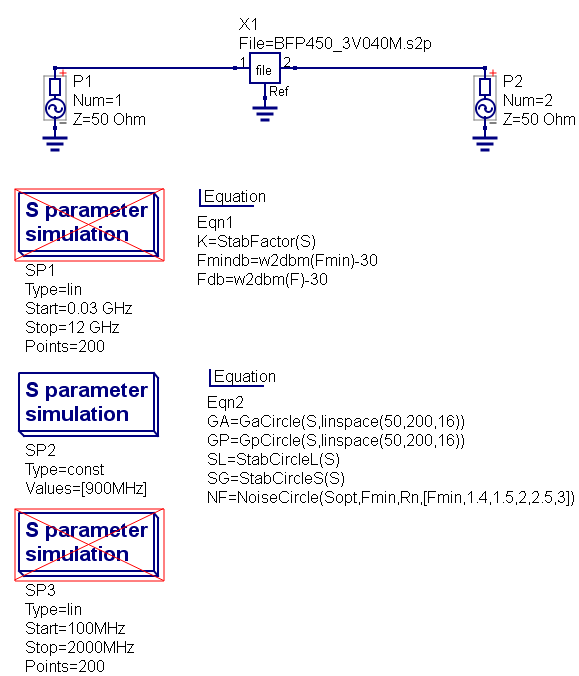
\includegraphics[width=8cm]{bfp450_1_sch.png}}
  \caption{Check the S-Parameters.}
  \label{fig:bfp450_1_sch}
\end{figure}


Now back to the real design (Fig.~\ref{fig:bfp450_1_sch}): In a first step,
we will use this file and observe the performance graphically. For
this proceed as follows:
\begin{enumerate}
\item Open a new project (e.g. {\tt S\_PARAM\_AMP})
\item open a new schematic (e.g. {\tt BFP450\_1.sch})
\item copy the a.m. .s2p-file into the project's directory
\item Set up a schematic ({\tt BFP450\_1.sch}) with 
  \begin{enumerate}
  \item two signal sources (as ports)
  \item one 2-port S-Parameter file component
  \item Equations
    \begin{itemize}
    \item $FmindB=w2dbm(Fmin)-30$
    \item $FdB=w2dbm(F)-30$
    \item $K=StabFactor(S)$
    \end{itemize}
  \item and an S-Parameter Simulation over the desired frequency range
    (e.g. 30\,MHz to 12\,GHz in 200 steps), with noise calculation
    enabled in the properties tab.
  \end{enumerate}
\end{enumerate}
The parameter $K$ is the stability factor. If it is larger than unity,
the device is absolutely stable and allows us to connect any passive
element at input and output, it will not oscillate. If $K$ is less
than one, some stability caution must be exercised. $FmindB$ is the
minimum noise figure (as taken from the .s2p-file). The equation
converts the QUCS-internal parameter $Fmin$, which is in linear scale,
in simple deciBels.

\begin{figure}
  \centering
%  \subfloat[]
  {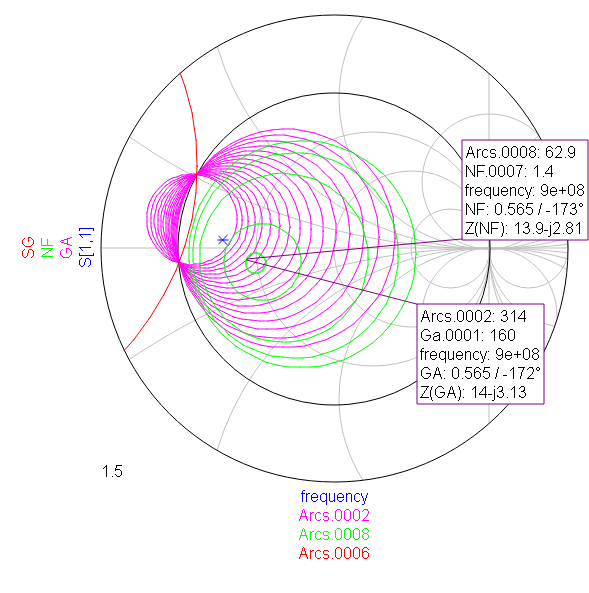
\includegraphics[width=10cm]{bfp450_1_source.png}}
  \caption{Source side parameters of the BFP450 with stability (red) and
    gain (purple) as well as noise (green) circles for different
    matching conditions. $S_{11}$ is a blue asterisk.}
  \label{fig:bfp450_1_source}
\end{figure}

Perform the simulation (Fig.~\ref{fig:bfp450_1_source}) and check at
least the parameters $S_{11},S_{22}$ in a Smith diagram, and $S_{21},
K, Fmindb$ in a rectangular diagram. We find $K>1$ above 1.3\,GHz,
which is nice, but requires us to check stability at the desired
frequency of 900\,MHz and below.

Note that we have connected the common port (emitter) of the
transistor directly to ground. This is usually not realistic, since in
order to ground it, at least two vias are required at the emitter. A
check will show, that these vias (in a thin 0.5\,mm substrate) will
not change the S-Parameters of the two-port too much, thus, for
simplicity, we will omit this step, but still note that in a practical
design this omission might be dangerous.

\tutsubsection{Choice of Gain, Noise and Reflection}

{\bf Caution:} When working with 'Circles' make sure you only have
one two-port with P1 and P2 (in- and output) in the schematic,
otherwise the equations may fail to work.

Gain, noise and reflection coefficients can be chosen. For the
time being we will focus only on the design frequency of 900\,MHz
and add to the design
\begin{enumerate}
\item S-Parameter simulation (called SP2) with one frequency (900\,MHz), and noise
  enabled.
\item equations (in a new equation-set)
  \begin{itemize}
  \item $GA=GaCircle(S,linspace(50,200,16))$
  \item $GP=GpCircle(S,linspace(50,200,16))$
  \item $SL=StabCircleL(S)$
  \item $SG=StabCircleS(S)$
  \item $N=NoiseCircle(Spot,Fmin,Rn,[Fmin,1.4,1.5,2,2.5,3])$
  \end{itemize}
\end{enumerate}
Now deactivate the first simulation (SP1) and start the simulation and
set up the following result plots:
\begin{itemize}
\item Smith-Diagram (range 0 to 1.5 with 5 steps) with
  $S_{11},SG,GA,NF$. $S_{11}$ should be asterisk or something similar.
\item Smith-Diagram (range 0 to 1.5 with 5 steps) with
  $S_{22},SL,GP$.  $S_{22}$ should be asterisk or something similar.
\end{itemize}
You will find a lot of circles in different colors (see
Fig.~\ref{fig:bfp450_1_source}), place markers to get more
information. For instance there is one small circle indicating all
source reflections leading to a noise figure of
$F=1.4(=1,46\,\einh{dB})$. That is what we want. This circle
intersects with the $GA$-circle with $G_A=160(=22\,\einh{dB})$ at two
positions. We will not chose a point closer to $S_{11}$ and the
instable region (that is the region that is not contained in the $SL$
source stability circle), because that would make stability an even
greater issue.

\begin{figure}
  \centering
%  \subfloat[]
  {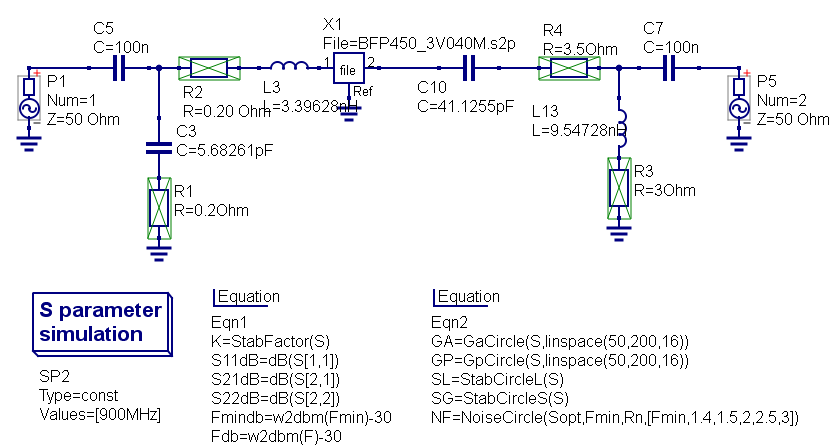
\includegraphics[width=12cm]{bfp450_1a_match.png}}
  \caption{Small signal (S-Parameter) circuit with matching
    networks. Resistors are ignored so far}
  \label{fig:bfp450_1a_match}
\end{figure}

\begin{figure}
  \centering
%  \subfloat[]
  {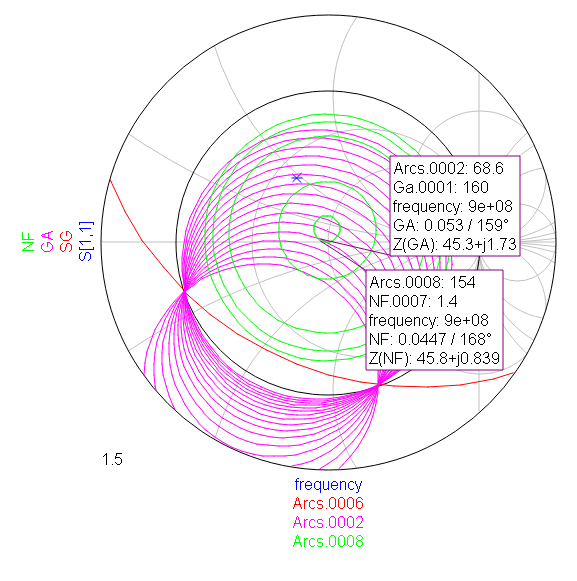
\includegraphics[width=10cm]{bfp450_1a_match_result.png}}
  \caption{Input side matching network results.}
  \label{fig:bfp450_1a_match_result}
\end{figure}


Since the difference between the two intersecting points is small, we
pick (from the marker field) $\Gamma_S(=GA)=0.565e^{-j172^\circ}$ as
the source reflection that we will present to the device. The input
matching circuit can be designed with the Matching Tool of
QUCS. However, since we want to transform the 50\,$\Omega$ port
impedance of P1 into the above reflection, the Matching-Circuit Tool
needs to be tricked. That is easy, we just calculate the matching
circuit for the complex conjugate (i.e. the negative angle) for it. It
is suggested to do these steps in a new schematic called {\tt
  BFP450\_2.sch}. The circuit is a simple LC-network
(Fig.\ref{fig:bfp450_1a_match}, left side), check if it works, if you
wish. A good check is to display the same Smith-chart (for the input
side) as mentioned above. Now, the $Gain=160,NF=1.4$-point should be
in the center of the diagram indicating, that a source with input
impedance 50\,$\Omega$ would give the desired result
(Fig.~\ref{fig:bfp450_1a_match_result}). So much for the input, still
the source stability circle intersects the SD with $|\Gamma|=1$. The
device is still only conditionally stable, we need to fix that later.

Next we will design the output matching network. A good choice may be
to conjugately match $S_{22}$ to 50\,$\Omega$. This can be done by
simply reading $S_{22}$ (you may want to use the marker), and use the
Smith tool, or by simply right-clicking on the marker information in
selecting 'power matching'. After the matching circuit has been
calculated incorporate it into the design (between output port of the
file-component and P2), be careful in order not to put it in the
wrong orientation. Re-simulation shows good output match and a gain of
about 22\,dB, as well as the desired operation at the input. 

\tutsubsection{Getting the Amplifier Stable at the Operation Frequency}

Still the amplifier has instable regions. That is the intersection of
the source or load stability circle and the $|\Gamma|=1$-boundary of
the Smith-Diagram (SD), that does not contain the center of the
SD. Incorporating some losses into the matching networks, especially
at the output will do the job. This may not be the most efficient and
most sophisticated way, maybe changing the matching circuits in a
purely reactive way or putting some line or reactance at the source
does a similar or better job.

Adding series resistances of $1/5\,\Omega$ at the input matching
elements helps and further inserting about $3.5\,\Omega$ series
resistance at the output moves the stability circles out of the SD
(Fig.~\ref{fig:bfp450_1a_match} with activated resistors).  But it
also drops the gain ($S_{21}$) from 160 to 130 (i.e. from 22\,dB to
21.2\,dB) and increases noise figure to 1.6\,dB. We will pay the price
of 0.8\,dB less gain and 0.15\,dB higher noise figure for stability.

Now we can do a simulation over the entire frequency range and see
that we have an amplifier with good gain, moderate noise, well matched
at the output, badly matched at the input.

\tutsubsection{The Biasing Network}

Further, we need to add the biasing network that, while not disturbing
anything at the operation frequency, serves two purposes
\begin{enumerate}
\item Set the DC-operation point of the device (i.e. make sure there
  is $V_{CE}=3\,\einh{V}$ and $I_C=40\,\einh{mA}$) and
\item stabilize the device at all frequencies apart from 900\,MHz.
\end{enumerate}

\begin{figure}
  \centering
%  \subfloat[]
  {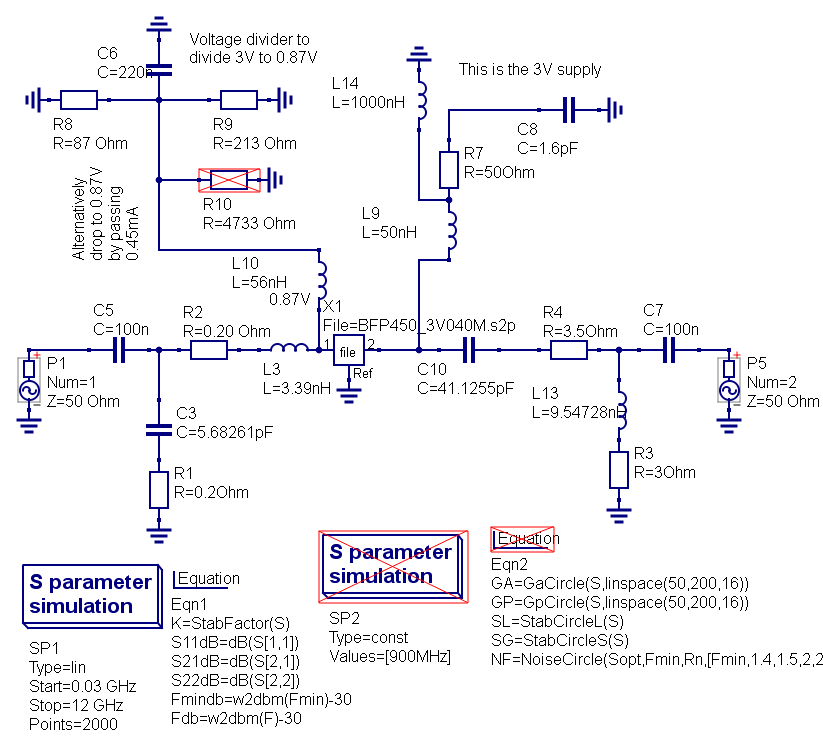
\includegraphics[width=12cm]{bfp450_2_sch.png}}
  \caption{Complete amplifier as small signal circuit.}
  \label{fig:bfp450_2_sch}
\end{figure}

\begin{figure}
  \centering
%  \subfloat[]
  {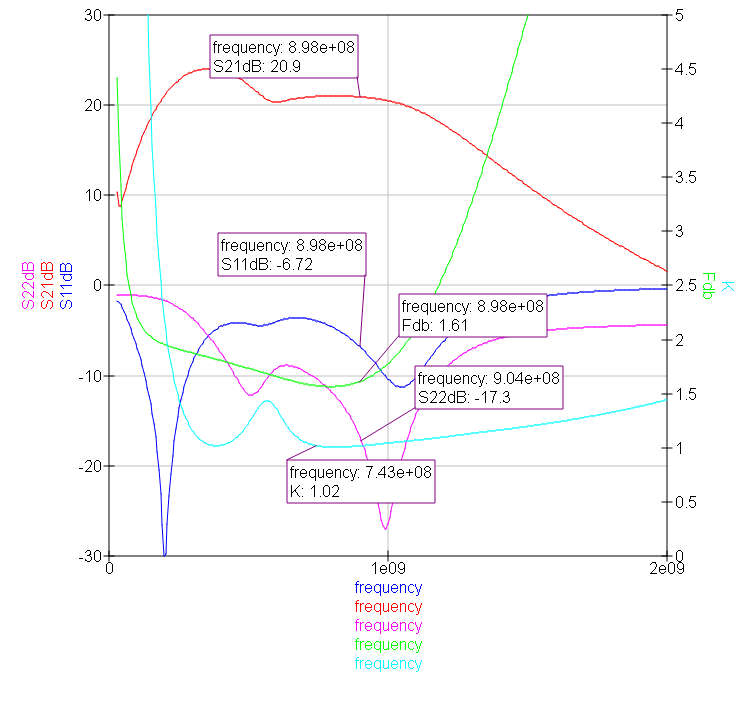
\includegraphics[width=10cm]{bfp450_2_result.png}}
  \caption{Performance of the entire amplifier.}
  \label{fig:bfp450_2_result}
\end{figure}

Starting with the output side we add a choke inductor and a series
resistor. Of course, the resistor is not wanted, it is, however,
needed in order to stabilize the amplifier at about 500\,MHz, where
$K<1$, initially. A choke inductor is the method of choice to
RF-decouple the supply network, we start off with a $L=50\,\einh{nH}$
RF inductor and set up a series resonator (resonant at about 500\,MHz)
with $C=1.6\,\einh{pF}$ and a series resistor of 50\,$\Omega$. That
should be (large $L$) invisible to 900\,MHz, but resonant at the
possible instable frequency around 500\,MHz. This signal, however, is
now directly routed to a 50\,$\Omega$ match. Effectively this does the
job of stabilizing the device, the 3\,V DC is then connected via a
choke (100\,nH or 1\,mH will do) to the a.m. inductor. Be aware of
parasitic capacitances in the inductor! The result can be found in
Fig.~\ref{fig:bfp450_2_sch}.

Let's turn to the input side: The datasheet helps. Figure 5-2 tells us
that around $V_{CE}=3\,\einh{V}$ $I_C$ does not depend much on
$V_{CE}$. Most notably, there is not much difference in current
between $V_{CE}=2\,\einh{V}$ and $V_{CE}=3\,\einh{V}$. This is
important to validate the following figures. There is a Base current
$I_B=0.38\,\einh{mA}\ldots0.57\,\einh{mA}$ at
$I_C=40\,\einh{mA}$. Let's estimate $I_B=0.45\,\einh{mA}$. Figure 5-4
gives the information that the Base-Emitter voltage must be
$V_{BE}=0.87\,\einh{V}$, and (Figure 5-5) the Base current is in the
same regime as estimated above. So, in order to generate 0.87\,V from
3\,V a voltage divider of 87:300 is in order. The current in the
divider must be larger (pick 20 times) than the base current in the
transistor, thus the dividers total resistance shall be not greater
than 333\,$\Omega$. We pick 300\,$\Omega$ and the divider is
$R_2=87\,\Omega$ and $R_1=213\,\Omega$ (not caring that these might
not be for sale). The voltage divider must be AC decoupled from Base
with a choke inductor of 56\,nH and the entire circuit should be DC
decoupled from the ports. Alternatively, the Base biasing can be done
with only one resistor of 4733\,$\Omega$ that has a voltage drop of
2.13\,V at a current of 0.45\,mA, also bringing 870\,mV to the
base. The latter choice might not be very stable if temperature
changes.

The overall performance of the amplifier with bias network and all is
depicted in Fig.~\ref{fig:bfp450_2_result}. For this tutorial we will
not worry about a few shortcomings, namely the shift of $S_{22}$
minimum towards a slightly too high frequency and the quite bad $S_{11}$
(input matching). This is due to the choice of good noise figure, but
basically means that only a little less then 80\,\% of the available
power will be 'permitted' to enter the amplifier, the rest is reflected.

\tutsubsection{The DC, AC or Spice Model}

To verify the a.m. design, a check with the Spice model shall be
done. Included in the set of S-Parameter files for the BFP450 there
comes a spice model (initially called ...txt). This includes a model
that should be generally able to describe the component and allow for
DC, AC, and transient analyses. 

\begin{figure}
  \centering
%  \subfloat[]
  {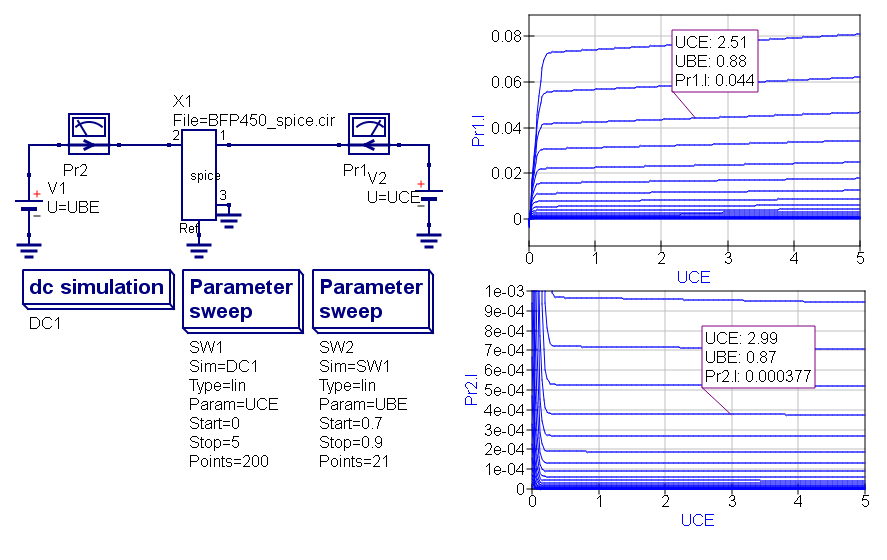
\includegraphics[width=12cm]{bfp450_dc.png}}
  \caption{DC analysis of the transistor BFP450.}
  \label{fig:bfp450_dc}
\end{figure}

In a first step, rename the .txt-file to .cir and then use the
'Circuit' from QUCS-file components in a new schematic (e.g. {\tt
  bfp450\_dc.sch}). Connect the component to the .cir-file and add 
DC-voltages $UBE$ and $UCE$ to Base (port 2) and Collector (port 1)
properly ground ref and port 1 as well as the supplies. Add current
probes in Base and Collector path. The simulation for DC operation
lines is set up as follows (Fig.~\ref{fig:bfp450_dc}):
\begin{itemize}
\item Use DC-Simulation DC1
\item Add Sweep SW1 and connect to DC1 with Param UCE from 0 to 5 V in
  200 steps. (This will be the inner parameter sweep loop)
\item the outer sweep-loop is performed by Sweep SW2, sim=SW1,
  PARAM=UBE from 0.7 to 0.9V with 21 points.
\end{itemize}
In the end, you will see the Collector current as a function of Base
and Collector voltage and Base current as the same. This is
essentially only a repetition of what we already know from the data
sheet (Fig.~\ref{fig:bfp450_dc}).

\begin{figure}
  \centering
%  \subfloat[]
  {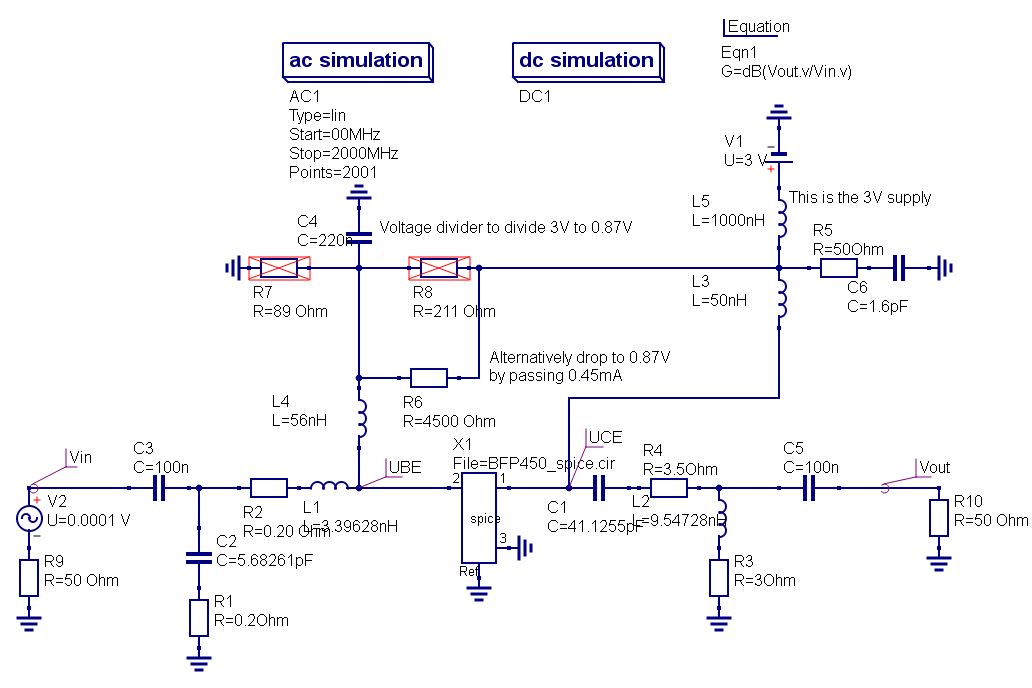
\includegraphics[width=12cm]{bfp450_ac_sch.png}}
  \caption{DC and small signal AC analysis of the completed amplifier.}
  \label{fig:bfp450_ac_sch}
\end{figure}

An AC-small signal analysis (Fig.~\ref{fig:bfp450_ac_sch}) shall be
used to verify the S-Parameter results. For this the entire
S-Parameter circuit including both matching and biasing networks shall
be copied to a new schematic (e.g. {\tt bfp450\_ac.sch}). The
S-Parameter 2-port must be replaced by a properly grounded 'Circuit'
file component and port one is replaced by an AC-source (V=0.0001\,V)
in series with 50\,$\Omega$. The output measurement port is replaced
by a 50\,$\Omega$ load. Both nodes (wires), the input to the input
matching network, and the wire at the output resistor shall be named
($Vin$ and $Vout$ for instance). A 3\,V DC-source is required at the
appropriate location, a few (RF) grounds must be deleted and the
input-side bias voltage divider and the output side bias-point must be
connected to the source. A DC-Simulation to find the DC operating
point and an SC simulation (e.g. from 100\,MHz to 2\,GHz) must be
included, an equation $G=dB(Vout.v/Vin.v)$ would calculate the pure
gain.

\begin{figure}
  \centering
%  \subfloat[]
  {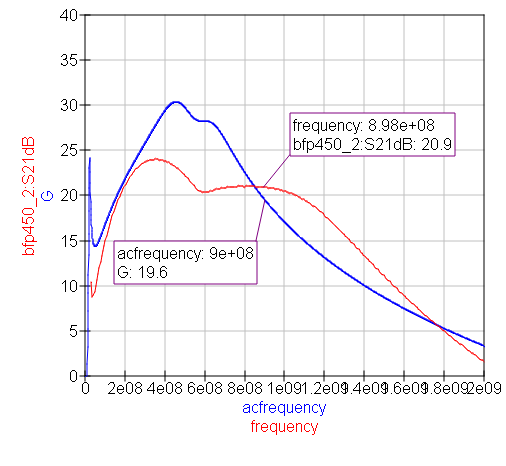
\includegraphics[width=8cm]{bfp450_ac_result.png}}
  \caption{Ratio of output to input voltage $(G)$ in blue of
    AC-analysis and $S_{21}$ (red) of S-Parameter simulation as
    measures of the gain.}
  \label{fig:bfp450_ac_result}
\end{figure}


Run the simulation and check (maybe in a table) the DC-operating point
with $VCE.V$ and $V1.I$ ($V1$ should be the 3\,V-DC-source). Adjust the
input side biasing voltage divider until the operating point is
correct. Now you might want to check $G$ as a function of frequency
and compare with $S_{21}$ from the previous S-Parameter
simulation. There is some, but by far not perfect agreement as shown
in Fig.~\ref{fig:bfp450_ac_result}.

A deeper look into the models will show that the measured S-Parameters
as they come from the vendor differ somewhat from the simulated
performance from the spice-model. Since S-Parameters are measured and
only valid for a much more special range of operation, I would trust
them a little more than the overall and do it all spice model.

\tutsection{S-Parameter Design of a Low-Noise 11\,GHz Amplifier}

Now that we have designed an amplifier with only lumped elements, we
may feel confident to use something more advanced. At the desired
frequency range for TV-satellites (i.e. 11GHz) lumped elements,
especially inductors, are not available with low enough
parasitics. However, microstrip lines are. So we will turn our
attention to a LNA that does not (at least in the matching network)
need inductors or capacitors, only microstrips suffice. For this need
to utilize an QUCS-external tool. The tool JSmith \cite{jsmith} lets
us move around in the smith chart. An alternative is a Excel-based
automatic calculator tool found at \cite{ibdrigodwn} after
registration and included in this package.

In the end, there should be a dual stage low noise amplifier.

\tutsubsection{1. Stage: Choice of Transistor,  DC-Bias and Ground Connection}

For some reason, maybe recommendation, we will pick the VMMK-1218 of
Avago \cite{avagovmmk1218} and find at their web-page all relevant
information. Some use has been made of the application notes
\cite{avago_an5385,avago_an5408}, for more and detailed information
the interested reader is referred to those. The data sheet suggests
that at 11\,GHz the biasing point of $V_{DS}=2\,\einh{V}$ and
$I_D=20\,\einh{mA}$ delivers good performance with
$F_{min}=0.78\,\einh{dB}, S_{21}=9.78\,\einh{dB}$ while exhibiting
only $20\,\einh{mW}$ of DC power requirement.

\begin{figure}
  \centering
%  \subfloat[]
  {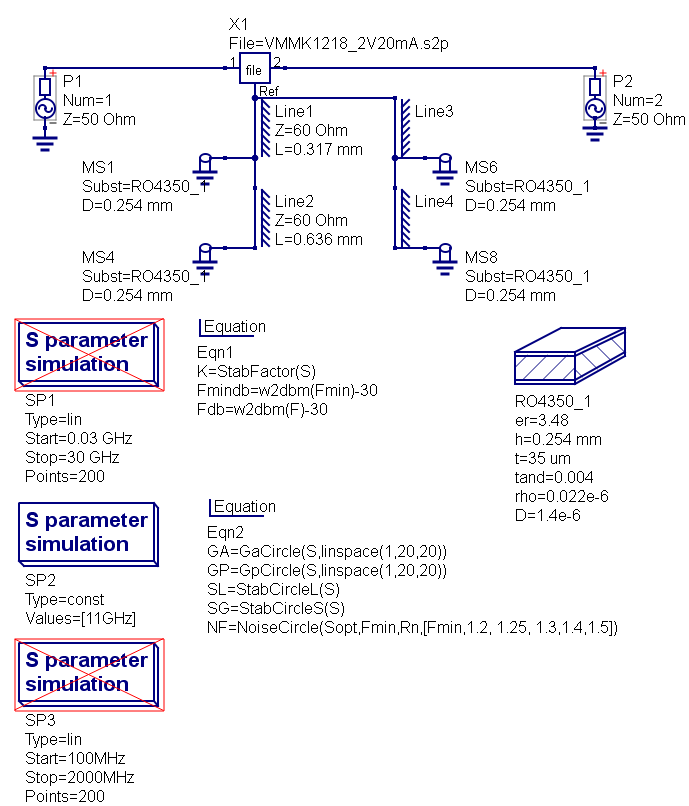
\includegraphics[width=8cm]{vmmk1218_1_sch.png}}
  \caption{Bare VMMK-1218 with ground connection at the source (as
    suggest in \cite{avagovmmk1218}.}
  \label{fig:vmmk1218_1_sch}
\end{figure}

Let's go for it and check the S-Parameters {\tt VMMK1218\_2V20mA}. A
quick check on the S-Parameters and stability shows that the device is
(slightly) conditionally stable ($K<1$) at 11\,GHz, stable above, but
just a mess at low frequencies. To simulate this, you may copy the
schematic {\tt bfp450\_1.sch} to {\tt vmmk1218\_1.sch} and adjust the
S-Parameter file as well as the frequency range. A first note of
caution is required here, since at 11\,GHz the wave is short, we will
not be able to connect the source to ground ideally. The recommended
land pattern is found on p.\,10 of the datasheet. This connection
should be modelled as early as possible since it severely affects the
S-Parameters and thus all subsequent calculations. Further, microstrip
lines do not work with noise calculations in the S-Parameter
simulation enabled, this seems to be a shortcoming in QUCS, so we need
to turn to ideal transmission lines. Now, we assume RO4350
($h=0.254\,\einh{mm}$) as a substrate (found in the QUCS-library), and
calculate the MS-lines to vias with the QUCS-Line Calculation. There
is a line with $W=0.4\,\einh{mm},\ l=0.2\,\einh{mm}$ that comes out as
$60\,\Omega, l_{el}=4^\circ$ and one with $l=0.4\,\einh{mm}$ that is
$l_{el}=8^\circ$ long. This models the source to ground connection
(Fig.~\ref{fig:vmmk1218_1_sch}), parallel as there are two sides and
appropriate vias connected (surprisingly these do not cause problems
in noise calculation).

\begin{figure}
  \centering
%  \subfloat[]
  {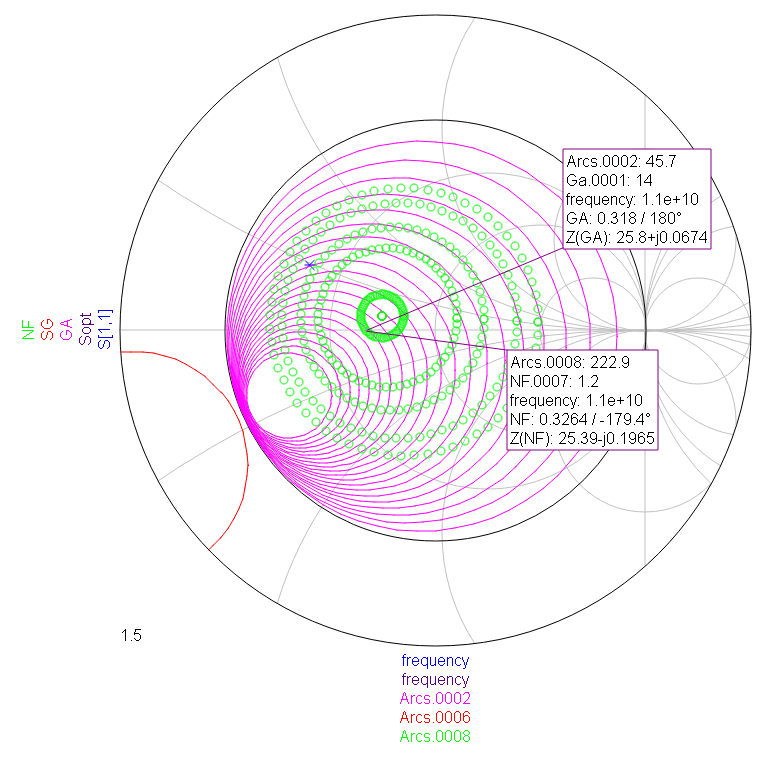
\includegraphics[width=12cm]{vmmk1218_1_source.png}}
  \caption{Input-side refleciont (blue), gain (purple), stability
    (red) and noise (green) conditions with modelling the ground at
    fet's source.}
  \label{fig:vmmk1218_1_source}
\end{figure}

The nice thing is, this feedback at the source (that's what it
essentially is) makes the device unconditionally stable at the
operation frequency, the bad thing is, it slightly deteriorates
performance (Fig~\ref{fig:vmmk1218_1_source}). 

\tutsubsection{1. Stage: Matching Networks}
\label{ch:match1}

\begin{figure}
  \centering
  \subfigure[]
  {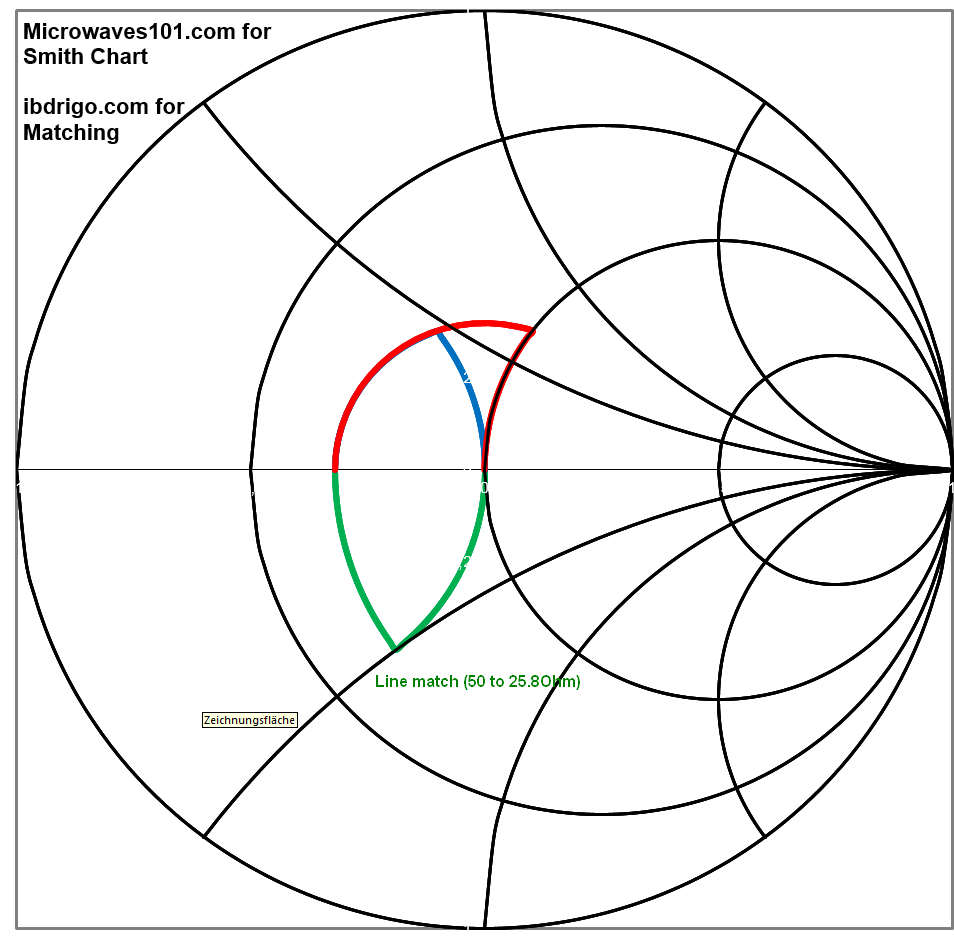
\includegraphics[width=6cm]{vmmk1218_input_match.png}}
  \subfigure[]
  {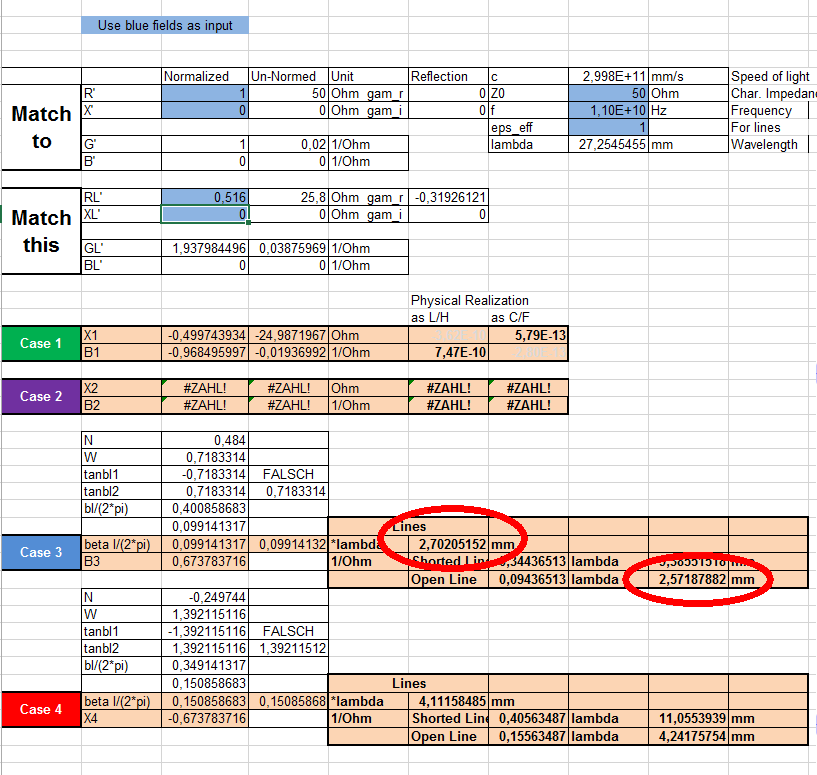
\includegraphics[width=8cm]{vmmk1218_input_match2.png}}
  \caption{Design of an input matching network with ideal transmission
    lines after \cite{ibdrigodwn}}
  \label{fig:vmmk1218_input_match}
\end{figure}

\begin{figure}
  \centering
%  \subfloat[]
  {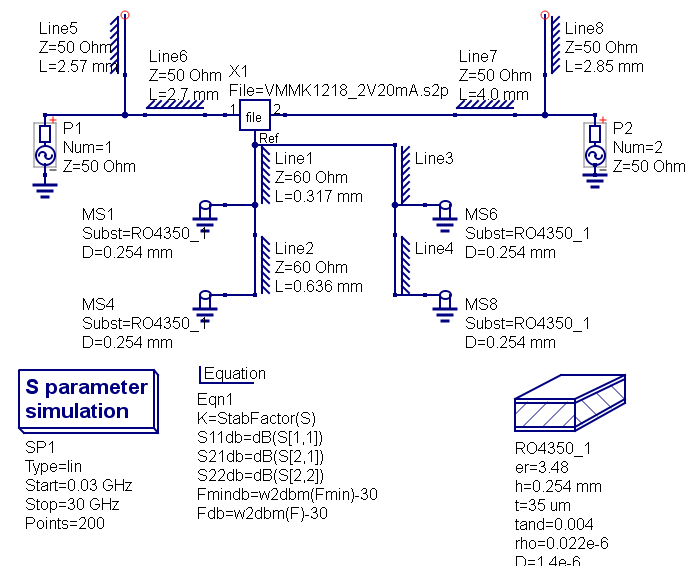
\includegraphics[width=12cm]{vmmk1218_matching.png}}
  \caption{The FET with matching networks.}
  \label{fig:vmmk1218_matching}
\end{figure}

\begin{figure}
  \centering
%  \subfloat[]
  {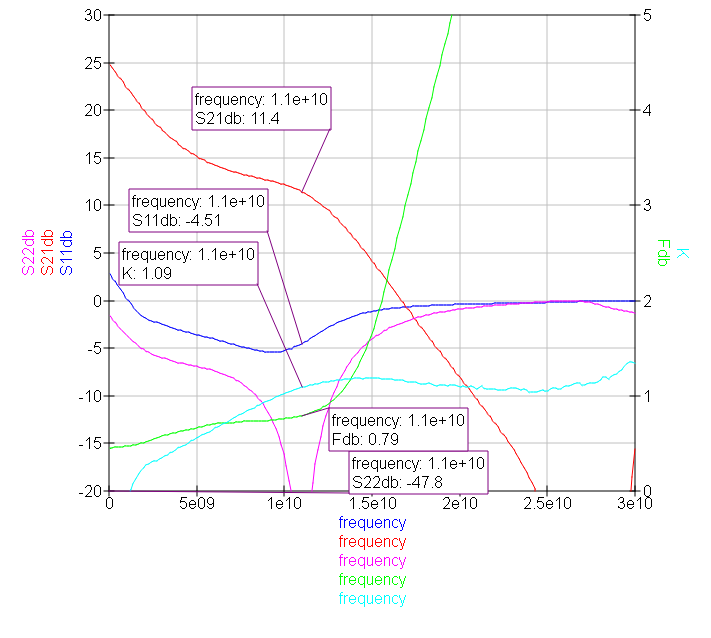
\includegraphics[width=8cm]{vmmk1218_match_result.png}}
  \caption{Result of the amplifier design with only matching networks.}
  \label{fig:vmmk1218_match_result}
\end{figure}

So in a new file {\tt vmmk1218\_2.sch}
(Fig.~\ref{fig:vmmk1218_matching}) the input and output match can be
designed. At input we go for noise figure of $F=1.2(=0.79\,\einh{dB})$
and $GA=14$ which requires transforming the $50\,\Omega$ signal source
to $\Gamma_G=-0.32$ (Fig~\ref{fig:vmmk1218_1_source}). The matching
circuit with using one of the a.m. external tools is now incorporated
at the input, the result is found in
Fig.~\ref{fig:vmmk1218_input_match}. At the output side we will
conjugately match to $S_{22}=-0.288-j0.215$, which (for the excel-tool
is an impedance of $Z_{out}=(25.5-j12.6)\,\Omega$). However, when
using this amplifier as a first stage in a dual stage amp, this needs
modification. The result over a wide frequency range is depicted in
Fig.~\ref{fig:vmmk1218_match_result}, it clearly shows the achievements
of $S_{21},S_{22}, F$ and the problems of $S_{11}$, which is due to
the choice of good noise figure and stability $K<1$ at low
frequencies.

\tutsubsection{1. Stage: Bias Network and Stabilizing}
\label{ch:bias1}

We select passive biasing of the Gate, that is, the Gate voltage is
simply derived from the supply (or Drain voltage) by a voltage divider
and some resistance at the main supply \cite{avago_an5385}. Again, the
Bias-network must be invisible for the operation frequency band. In
this case, two quarter-wavelength line-pieces are used. The first is
open at the end, and thus transforms the open into a short. At this
short we can do what ever we want, for example connecting a power
supply without changing anything (for the frequency of
operation). This is, because whatever we connect, it is in parallel to
a short. 

The second quarter-wavelength line-piece transforms the short (in
parallel to whatever) into an open at the location of the signal
line. Thus, the entire bias-network is invisible at the frequency of
operation. However, very well visible at other frequencies. For
example (and for problem) at half the operation frequency the two
quarter-wavelength pieces are not half-wavelength, but one
quarter-wavelength long. Without connecting something in the middle
between the line pieces, now the open is transformed into a short at
the signal line, effectively shortening the transistors input and/or
output at this frequency. This causes trouble, and may lead to
oscillation of the transistor.

In order to adjust the DC-operation point, at the input side a simple
voltage divider ($2450\,\Omega,\ 550\,\Omega$) derives the gate
voltage of $0.55\,\einh{V}$ (see datasheet Fig.~1) from the 3\,V
supply. Since the gate current is very small, a resistor of
$50\,\Omega$ can be used to connect the gate voltage. A cap 
RF-grounds the resistor on the other side and thus both provide a perfect
resistive match for low frequencies at the input of the FET.

\begin{figure}
  \centering
%  \subfloat[]
  {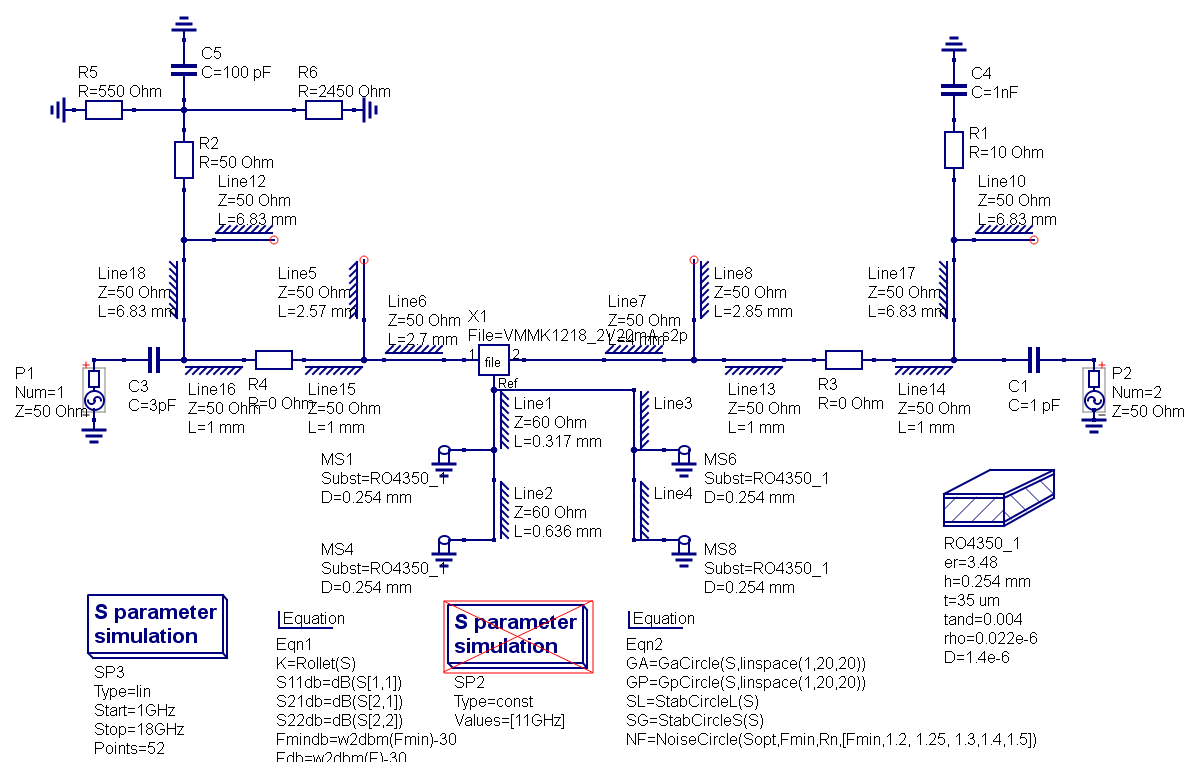
\includegraphics[width=12cm]{vmmk1218_3.png}}
  \caption{VMMK-1218 as single stage amplifier with matching and
    biasing.}
  \label{fig:vmmk1218_3}
\end{figure}

\begin{figure}
  \centering
  \subfigure[]
  {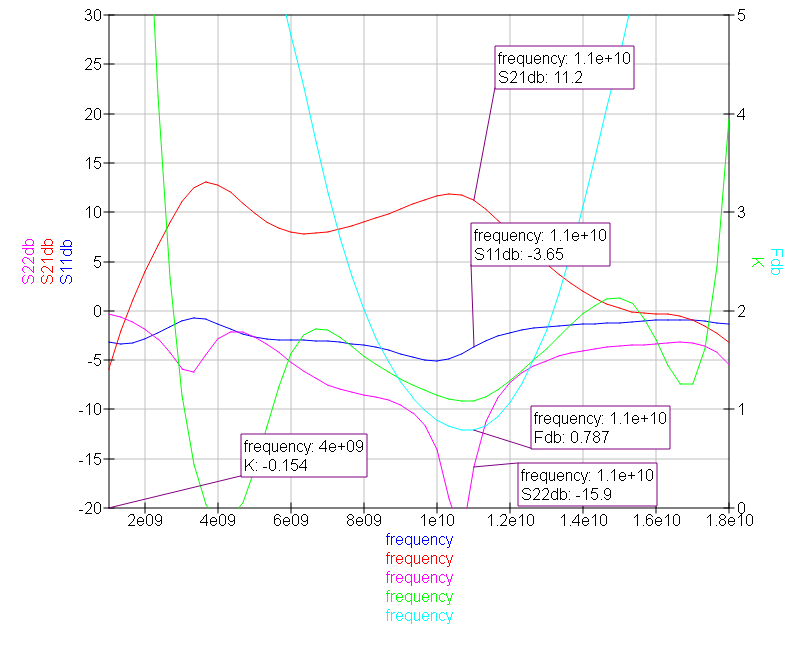
\includegraphics[width=7.5cm]{vmmk1218_3_result.png}}
  \subfigure[]
  {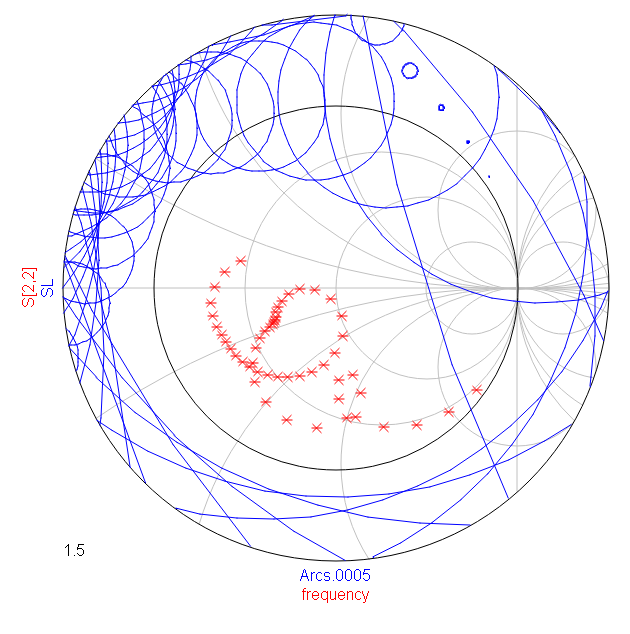
\includegraphics[width=7.5cm]{vmmk1218_3_result_b.png}}
  \caption{VMMK-1218 as single stage amplifier: Results overview (a)
    and detail (b) $S_{22}$ (red) and stability circles (from 1 to
    18\,GHz) (blue).}
  \label{fig:vmmk1218_3_result}
\end{figure}


At the output (Drain) side basically the same applies, except, no
voltage divider is needed to derive the Drain voltage and the resistor
should be as small as possible, since the entire Drain current is
flowing through it, causing quite some power loss and voltage drop
that needs to be compensated by a higher voltage from the supply.

Further, blocking capacitors are introduced, which, if small enough,
can help stability in the several GHz-range.

In Fig.\ref{fig:vmmk1218_3} the entire (idealistic) schematic is shown
and Fig.~\ref{fig:vmmk1218_3_result} depicts the results. It is clear
from Fig.~\ref{fig:vmmk1218_3_result}(a)
that the amplifier is massively (potentially) unstable around
4\,GHz. This is further underlined in (b), where some of the load
stability circles intersect the Smith Diagram. Check by yourself the
source side and play around with the resistors in the signal path and
see at what values (and resulting performance in $F$ and $S_{21}$ this
amplifier would be absolutely stable. Absolute stability at all
frequencies would be a requirement for an amplifier, that should be
sold on its own, since the customer may connect something to it and
does not want the amplifier to break. To this end, this amplifier
would not be saleable. 

\tutsubsection{2. Stage: Choice of Transistor and Bias Point}

The goal is to develop a dual stage amplifier at 11\,GHz with low
noise figure. The first stage is done, however unstable at some
frequency. For the second stage a different transistor will be
used. This is the ATF-36163 of Avago Technologies
\cite{avagoatf36163}. The main reason may be price: The VMMK-1218 is
about three times the price of the ATF-36163. We pick the same
Drain-Source voltage of $V_{DS}=2\,\einh{V}$ and a Drain current of
$I_D=20\,\einh{mA}$. It is not described in the data sheet, but
S-parameters are available. The corresponding Gate-Source voltage
$V_{GS}$ cannot be calculated from the given information, it must be
determined experimentally or from other simulations. It is probably
slightly negative (which is a disadvantage) or even zero or very close
to zero.

The source must be as well connected to ground as possible. The
footprint as given in the datasheet is used and the same substrate as
before is used. The circuit can be found in {\tt atf36163\_1.sch} and
is depicted later in Fig.~\ref{fig:dual1_sch}.

\tutsubsection{2. Stage: Matching Circuits}

The amplifier is absolutely stable at 11\,GHz and we go for
maximum gain and optimum match, because in a chain of amplifiers the
first stage determines the noise figure. So we have some more freedom
here. Hence the (optimum) input reflection of the second stage must be
complex conjugately matched to the output reflection of the first
stage (this is of course without the previously designed matching
network to $50\,\Omega$).

\begin{figure}
  \centering
  \subfigure[]
  {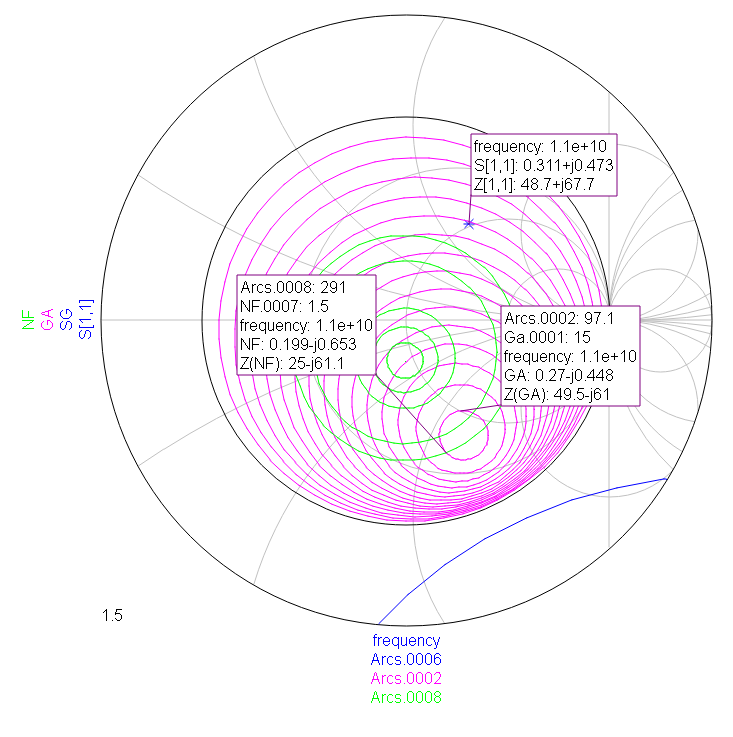
\includegraphics[width=7.5cm]{atf36163_input.png}}
  \subfigure[]
  {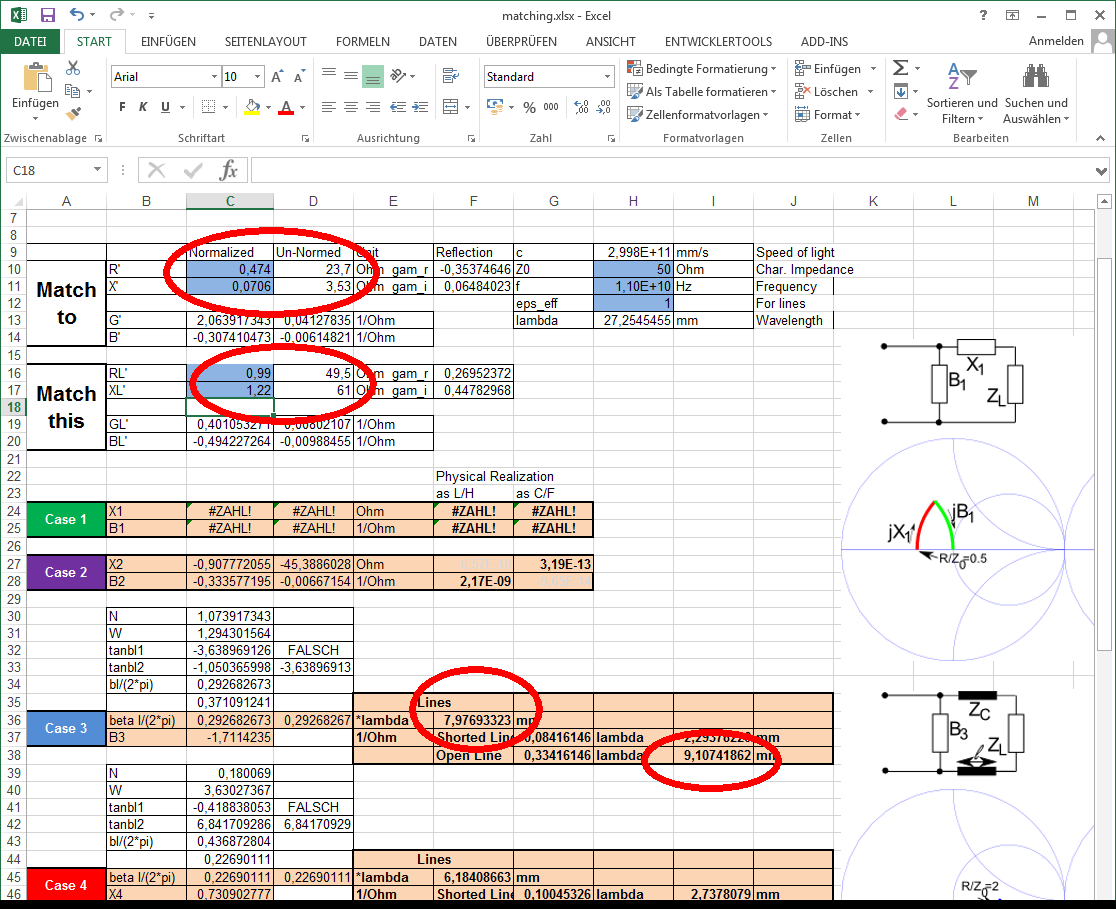
\includegraphics[width=7.5cm]{dual_match_interm.png}}
  \caption{Input impedance for optimum gain of the ATF-36163 (a) and
    matching it to the output of the VMMK-1218 (b)}
  \label{fig:atf36163_input}
\end{figure}

For geometrical reasons a $1\,\einh{mm}$ line has been added at input
and output of the FETs.  The input to ATF-36163 for optimum gain
(which is about 15) is (Fig.~\ref{fig:atf36163_input}(a)) and is about
$Z(GA)=(48.5-j61)\,\Omega$.  The output impedance of the first stage
is already known to be $Z_{out}=(25.5-j12.6)\,\Omega$
(Section~\ref{ch:match1}), but the added $1\,\einh{mm}$ line makes it
to $Z_{out}=(23.7-j3.53)\,\Omega$. For calculating the intermediate
match, the Excel-Tools is required. The impedances are plugged in with
positive imaginary part because of (1) matching in reverse direction
and (2) matching to complex conjugate
(Fig.~\ref{fig:atf36163_input}(b)). The resulting series line is
divided into two section, in order to place some cap as DC decoupling
there.

Next, the output match of the entire amplifier has to be
designed. Here, it turns out the overall $S_{22}$ is already close to
the origin of the Smith diagram and its real part is already about
$50\,\Omega$. To match the remaining imaginary part, a quite long
(about $12\,\einh{mm}$) open stub would be required. However, this
match would be better off with just a series capacitor of about
$1\,\einh{pF}$. Since we need that anyway for blocking, we just go that
route. 

\tutsubsection{The Final Bias Networks and Performance}

Next, all the bias networks are added, as explained in detail in
section~\ref{ch:bias1}. The gate of the ATF-36163 will require a
separate feeding, since it may be negative, so no divider is planned
here. The rest is the same as before, the resistors in the supply
(Drain) patch will be chosen as small as possible. It turns out that
$2\,\Omega$ suffice for stability.

\begin{figure}
  \centering
%  \subfloat[]
  {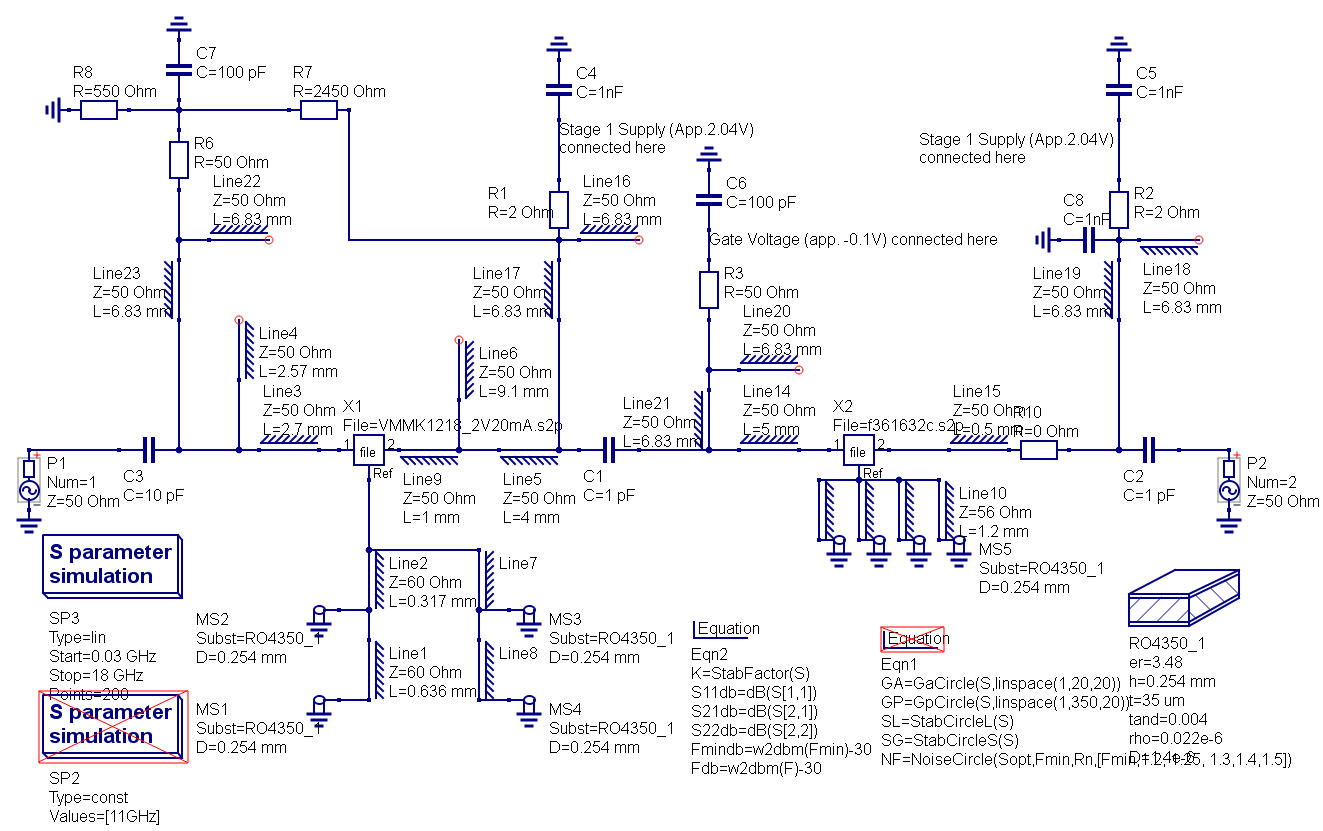
\includegraphics[width=12cm]{dual1_sch.png}}
  \caption{Schematic of the dual stage amplifier.}
  \label{fig:dual1_sch}
\end{figure}

\begin{figure}
  \centering
%  \subfloat[]
  {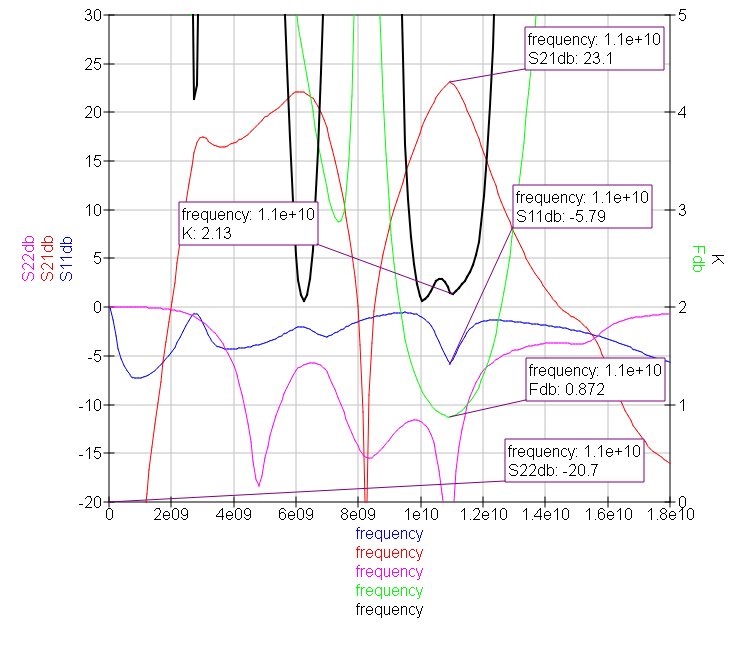
\includegraphics[width=8cm]{dual1_result.png}}
  \caption{Results of the dual stage amplifier design with ideal
    transmission lines.}
  \label{fig:dual1_result}
\end{figure}

The schematic {\tt dual\_1.sch} is shown if Fig.~\ref{fig:dual1_sch}
and results are in Fig.~\ref{fig:dual1_result}. The amplifier is
absolutely stable at all frequencies, noise figure is below
$0.9\,\einh{dB}$, output match almost perfect (better that
$20\,\einh{dB}$ and $S_{21}=23.1\,\einh{dB}$. Only the input match is
bad and around $5\,\einh{dB}$, which is the price to pay for the good
noise figure. 

\tutsection{Design in Microstrip}

The last step is to translate the design into a microstrip PCB
design. Noise calculation must be turned off, because it is not
supported in microstrips.

\begin{figure}
  \centering
%  \subfloat[]
  {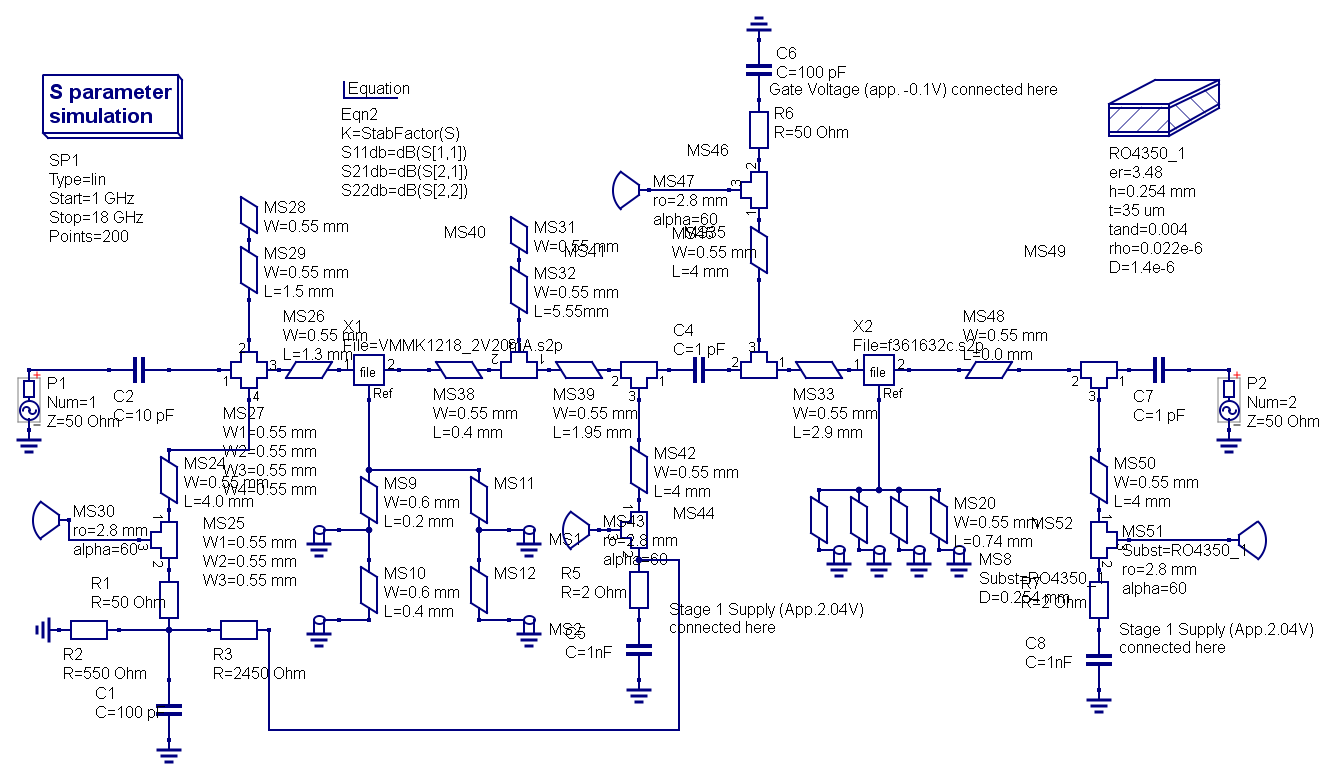
\includegraphics[width=12cm]{dual2_sch.png}}
  \caption{Schematic of the dual stage amplifier with microstrip lines.}
  \label{fig:dual2_sch}
\end{figure}

\begin{figure}
  \centering
%  \subfloat[]
  {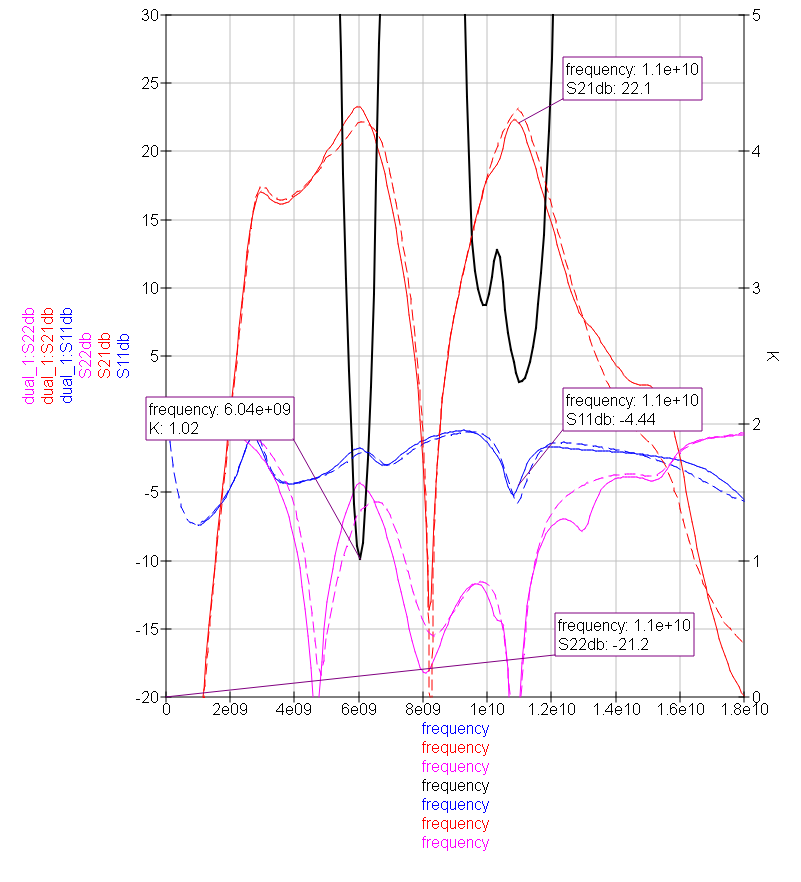
\includegraphics[width=12cm]{dual2_result.png}}
  \caption{Results of the dual stage amplifier design with microstrip 
    transmission lines.}
  \label{fig:dual2_result}
\end{figure}


The QUCS-Transmission line tool synthesizes that a $50\,\Omega$
microstrip line on RO4350 with $h=0.254\,\einh{mm}$ has a width of
$w=0.55\,\einh{mm}$ and an $\epsilon_r=2.64$. Thus, all ideal
transmission line lengths must be reduced by a factor of $1.625$. This
is a good starting point, but the translation from ideal to microstrip
lines must be done very carefully and network by network. The best
method is to stepwise exclude parts of the networks (e.g. the biasing
networks) and compare the ideal realization in $S_{21},\ S_{11},\
S_{22}$ and adjust the microstrip line length accordingly.

At last, replace all ideal networks by more realistic ones and maybe
fine-tune a bit. In this case, after replacement the amplifier got
only conditionally stable at around 5\,GHz, which required some
increase of length in the intermediate matching network. 

The final layout is shown in Fig.~\ref{fig:dual2_sch} and the results
are in Fig.~\ref{fig:dual2_result}. The results are in very acceptable
agreement with the ideal results. Of course, the gain has dropped a
little bit, since now there are losses in the lines. Unfortunately,
the noise figure could not be calculated while using microstrip
lines. However, since all other parameters fit well, the noise figure
should not deviate too much.

\tutsection{Conclusion}

It has been shown, how QUCS can be used to develop RF low noise
amplifiers, where vendor data on S-Parameters is available. To start,
a design in the sub-GHz regime utilizing only lumped components is
used as an introduction. Here, only QUCS-provided tools are used,
special attention is paid to use of circles (for gain, noise, and
stability) in the operation frequency band. The necessity of absolute
stability everywhere is emphasized and bias networks are designed to
enforce this. 

In a second example, design of a 11\,GHz  dual stage low noise amplifier for use
e.g. in direct broadcasting satellite applications is
demonstrated. Some steps from sub-GHz amplifier design are repeated,
some new aspects are introduced such as: Matching and biasing
networks based on transmission lines instead of capacitors and
inductors. Furthermore, the question of stability is much more severe,
and absolute stability can only be guaranteed in the dual stage
design, here. At last, the schematic parameters are translated into
manufacturable microstrip topology. For this design Excel-based tool
of the authors needs to be used. 

Overall, it has been demonstrated that QUCS can well be used to
develop linear amplifiers in different technologies. 


\begin{thebibliography}{1}
\bibitem{qucs}	 { Michael Margraf and Stefan Jahn and Jens Flucke and Raimund Jacob and Vincent Habchi and Toyoyuki Ishikawa and Gopala Krishna A  and Mike Brinson  and Helene Parruitte and Bastien Roucaries and  Gunther Kraut and Andrea Zonca },	 {Quite Universal Circuit Simulator (QUCS)},
   {2013},
   \url{http://qucs.sourceforge.net/},
   {called on 2013-01-16}

\bibitem{col91}
 {R. E. Collin},
 {Foundations for Microwave Engineering},
 {McGraw Hill},
 1991,
 2nd Ed.


\bibitem{poz05}
  {David M. Pozar},
   {Microwave Engineering},
  {John Wiley and Sons},
  2005,
  3rd Ed.

\bibitem{infbfp450}
  {Infineon},
  {BFP450},
  {2014},
  \url{http://www.infineon.com/cms/de/product/rf/rf-transistor/high-linearity-si-and-sigec-transistor-for-use-up-to-6-ghz/BFP450/productType.html?productType=db3a3044243b532e0124c9ced1886365},
  {called on 2014-11-09}


\bibitem{jsmith}
  {Besser Associates}, 
  {Scott Forbenius},
  {JSmith},
  {2014},
  \url{http://www.bessernet.com/jobAids/jSmith/jSmith.html},
  {called on 2014-11-09}


\bibitem{ibdrigodwn}
  {Gerald Oberschmidt},
  {Excel-Matching Tool},
  {2014},
  \url{http://ibdrigo.com/download1.php},
  {called on 2014-11-09}


\bibitem{avago_an5408}
  {Avago Technologies},
  {Using the VMMK-1218 Wafer Scale Packaged Enhancement Mode PHEMT 
in a 10 GHz Low Noise Amplifier, Application Note 5408},
  {2010},
  \url{http://www.avagotech.com/pages/en/rf_microwave/transistors/fet/vmmk-1218/},
  {called on 2014-11-09}


\bibitem{avago_an5385}
  {Avago Technologies},
  {VMMK-1218 Application Information, Application Note 5385},
  {2010},
  \url{http://www.avagotech.com/pages/en/rf_microwave/transistors/fet/vmmk-1218/},
  {called on 2014-11-09}


\bibitem{avagovmmk1218}
  {Avago Technologies},
  {VMMK-1218},
  {2014},
  \url{http://www.avagotech.com/pages/en/rf_microwave/transistors/fet/vmmk-1218/},
  {called on 2014-11-09}


\bibitem{avagoatf36163}
  {Avago Technologies},
  {ATF-36163},
  {2014},
  \url{http://www.avagotech.com/pages/en/rf_microwave/transistors/fet/atf-36163/},
  {called on 2014-11-09}


\end{thebibliography}
